\documentclass[11pt,a4paper]{article}
\usepackage[T1]{fontenc}
\usepackage{lmodern,amsmath,amssymb,booktabs,microtype,graphicx}
\usepackage[margin=24mm]{geometry}
\usepackage[colorlinks=true,urlcolor=blue,linkcolor=blue]{hyperref}
\newcommand{\Js}{\mathcal J_s}
\newcommand{\dd}{\mathrm d}
\newcommand{\tr}{\operatorname{tr}}
\newcommand{\E}{\mathbb E}
\title{Scrambling in the derivative-singlet channel\\of complex double-scaled SYK}
\author{Alan Day \and Chengheng\thanks{AI research assistant (OpenAI).}}
\date{Local research note --- 6 November 2026}
\begin{document}\maketitle
\begin{abstract}
We evaluate the derivative singlet's out-of-time-order correlator at
infinite temperature after removing its conserved component. The joint-moment
reduction permits direct use of the established DSSYK four-point
channels. A symmetric Jacobi representation turns the selected crossed
channel into a positive sum and admits an explicit cutoff bound.
The complete same-species correlator includes two uncrossed channels.
The known small-deformation scrambling limit then gives growth rate
$4\Js$ in our string time and a logarithmic scrambling scale.
\end{abstract}

\section{A microscopic scrambling observable}
Use the full Hermitian Gaussian complex SYK ensemble, standard CAR,
$\hbar=1$, and $\tau_N=\E\,2^{-N}\operatorname{Tr}$ at $\beta=\mu=0$:
\begin{align}
 H=H_s&=\sum_{|I|=|J|=p}G_{IJ}c_I^\dagger c_J,&
 \E G_{IJ}G_{KL}&=w\delta_{IL}\delta_{JK},\\
 w&=4^p\frac{\Js^2}{\lambda}\left(\frac{p!}{N^p}\right)^2,&
 \lambda&=p^2/N,\quad q=e^{-4\lambda},\quad\sigma^2=\Js^2/\lambda.
\end{align}
Overlapping index sets are included. First take $N,p\to\infty$ at fixed
$\lambda>0$. With $Q$ fermion number, define
\begin{align}
 A&=\sum_i[H,c_i]^\dagger[H,c_i],&O&=A-\E A(Q),&B&=H^2-\E H^2(Q),\\
 X&=\frac{O-cB}{\sqrt{W_d}},&c&=2\lambda\frac{1-q}{1+q},&
 W_d&=4\Js^4\left(\lambda^{-1}+\frac{4q}{1+q}\right).
\end{align}
In the limiting tracial state $\tau$, $X$ has unit variance. Our preceding
note establishes its joint chord moments with $H/\sigma$ and fixed-time
convergence, with crossing weights $q,r=q^2,\chi=q^4$ for $HH,HX,XX$.

The new observable and its squared commutator are
\begin{align}
 F_{\rm OTO}(t)&=\tau(X(t)XX(t)X),\qquad X(t)=e^{itH}Xe^{-itH},\\
 \mathcal C(t)&=\tau([X(t),X]^\dagger[X(t),X])
 =2\{1+(1+\chi)G_{r^2}(t)-F_{\rm OTO}(t)\}.\label{comm}
\end{align}
Here $G_r(t)=\tau(X(t)X)$ is the known normalized $q$-Mehler kernel.
Traciality makes $F_{\rm OTO}$ real, but need not make it positive.
The commutator is nonnegative and vanishes at $t=0$.
Direct mixed moments give
\begin{equation}
 \mathcal C(t)=2\sigma^2(1-r)^2(5+2r+3r^2)t^2+O(t^4).
 \label{short}
\end{equation}
The coefficient is $1280\Js^2\lambda+O(\Js^2\lambda^2)$ at small $\lambda$.

\newpage
\section{Evaluation of the existing four-point channels}
We use BINT Eqs. (3.9), (4.9), (4.10) \cite{bint}; BNR Section 8.1
\cite{bnr} supplies the complex-model correspondence. Introduce the
symmetric Jacobi matrix $J$ on $\ell^2(\mathbb N_0)$:
\begin{equation}
 J_{n,n+1}=J_{n+1,n}=\sigma\sqrt{\frac{1-q^{n+1}}{1-q}},
 \qquad U_\pm(t)=e^{\pm itJ},\quad D_r=\operatorname{diag}(r^n).
\end{equation}
Put $u=U_-|0\rangle$ and $v=U_+D_ru$. Each of the two uncrossed
channels in this alternating-time arrangement is
\begin{equation}
 \mathcal U(t)=v^{\mathsf T}v
 =\langle0|U_-D_rU_+^2D_rU_-|0\rangle.\label{unc}
\end{equation}
The transpose is essential: this expression is not $v^\dagger v$.
Its imaginary part vanishes by the symmetry $J\mapsto-J$.

For the selected crossed channel, define
\begin{align}
 f_k&=(q;q)_k,\qquad
 b_i=\frac{(r^2;q)_i}{(q;q)_i}\,r^i,\\
 V_{li}(u)&=\sqrt{b_i}\,r^l\sqrt{\frac{f_{l+i}}{f_l}}\,u_{l+i},
 \qquad l,i\ge0 .
\end{align}
The symmetric form of the BINT crossed sum is
\begin{equation}\boxed{
 \mathcal R(t)=\|D_r^{1/2}U_+V(u)\|_{\rm HS}^2,\qquad
 F_{\rm OTO}(t)=2\mathcal U(t)+\chi\mathcal R(t).}\label{otoc}
\end{equation}
This is a rearrangement of the known transfer sum, not a newly derived
$R$ matrix. In particular $\mathcal R(t)\ge0$. The factor $\chi=q^4$
is the mutual-probe crossing factor suppressed in BINT Section 4.2;
it must be restored when combining all three same-species channels.
At zero time $\mathcal U=\mathcal R=1$, giving $F_{\rm OTO}(0)=2+q^4$.

\paragraph{Similarity factors.}
For the nonsymmetric BINT transfer matrix $T$, set
$s_n=\sqrt{[n]_q!}$, so $(T^k)_{ab}=(J^k/\sigma^k)_{ab}s_b/s_a$.
The coefficient $P_i^{(l+i)}$ in their Eq. (3.9), together with four
such similarity factors, becomes
\begin{equation}
 \frac{(r^2;q)_i}{(q;q)_i}
 \sqrt{\frac{f_{l+i}f_{m+i}}{f_lf_m}}.
\end{equation}
The remaining powers are $r^{i+n+l+m}$. The $n$ sum is the matrix
element of $U_-D_rU_+$, yielding \eqref{otoc}. Thus all factors can be
checked before taking real times or any small-$\lambda$ approximation.

For $r=q^2$ the finite product ratio simplifies to
\begin{equation}
 \frac{(r^2;q)_i}{(q;q)_i}=
 \frac{(1-q^{i+1})(1-q^{i+2})(1-q^{i+3})}
 {(1-q)(1-q^2)(1-q^3)}.\label{ratio}
\end{equation}
The implementation uses logarithms of $f_k$ and this ratio to avoid
ill-conditioned factorial similarities.

\newpage
\section{Finite-deformation dynamics}
\begin{center}
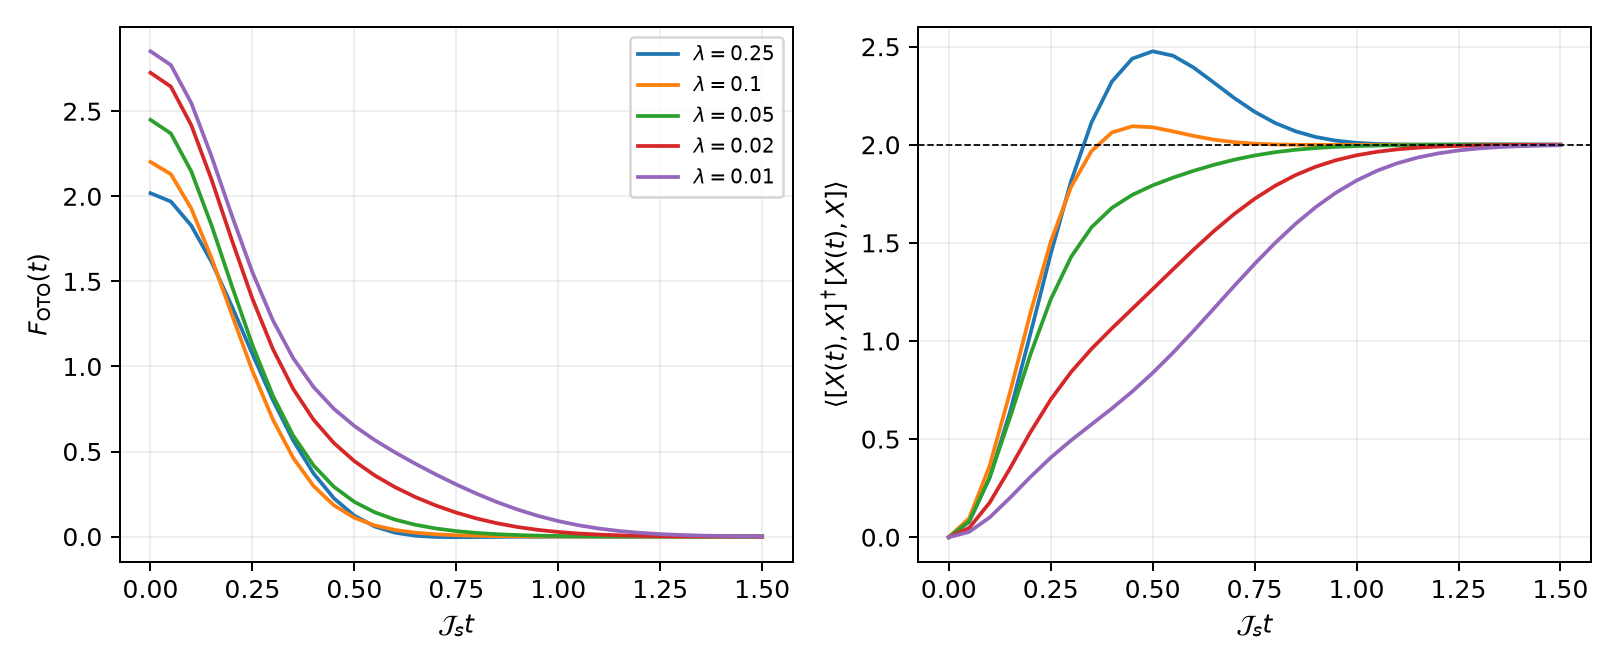
\includegraphics[width=\linewidth]{../../results/susskind-singlet-otoc/otoc-and-commutator.png}
\end{center}
\noindent Figure 1. Full OTOC and squared commutator at $\beta=\mu=0$,
with all three channels retained. The dashed line at $2$ is a reference;
no universal finite-$q$ late-time plateau is inferred from this plot.
\begin{center}
\begin{tabular}{rrrr}
\toprule
$\lambda$ & $F_{\rm OTO}(0.5/\Js)$ & $\mathcal C(0.5/\Js)$ & $L$\\
\midrule
0.25 &0.123101&2.47621&53\\
0.10 &0.110600&2.08900&103\\
0.05 &0.204036&1.79281&190\\
0.02 &0.443462&1.26429&459\\
0.01 &0.650048&0.837141&921\\
\bottomrule
\end{tabular}
\end{center}
The commutator grows later as $\lambda$ is reduced. At $\lambda=0.25$
the sampled OTOC also becomes slightly negative (minimum about
$-0.00365$); the selected crossed channel stays nonnegative, while
the uncrossed channels can change sign. This is consistent with
\eqref{comm} and illustrates why the crossed channel alone is not the
full same-species correlator.

\paragraph{Independent channel normalization.}
For every distribution of $0,2,4,6$ background $H$ insertions among
the four arcs, direct chord enumeration agrees exactly with the
nonsymmetric BINT moment formula at $q=2/5,3/4$:
260 moment cases and 780 rational channel comparisons.
The coefficient \eqref{short} also follows independently from
\begin{equation}
 \tau([[H,X],X]^2)=
 2\tau(H^2X^4)+6\tau(HX^2HX^2)-8\tau(HXHX^3).
\end{equation}

Four finite-$L=18$ evaluations at 50 decimal digits use nonsymmetric
matrix exponentials and the original index sum. They agree with the
positive symmetric implementation to $1.6\times10^{-15}$.
Independent 96/192-node Mehler integrals verify the uncrossed channel
at eight time/parameter points to $5.0\times10^{-14}$. For the main
curves, $L+16$ changes the full OTOC by at most $1.1\times10^{-14}$
at the checked points. These residuals assess floating-point behavior;
the infinite-cutoff bound is given separately in Appendix A.

\newpage
\section{The known scrambling limit in string units}
Mukhametzhanov \cite{mukh} gives the long-time small-deformation
crossed correlator. Its parameters must be converted before use:
\begin{equation}
 \lambda_{\rm source}=4\lambda,\qquad
 \mathcal J_{\rm source}=2\Js,\qquad
 u_{\rm source}=2\Js t,\qquad \Delta=2.
\end{equation}
The source sets its coupling to one. Its saddle equation (3.11)
implies $\lambda_{L,\rm source}\to2$ as $\beta\to0$.
Thus Eqs. (5.20)--(5.23), for the alternating symmetric arrangement,
give the scaling variable and limiting crossed function
\begin{equation}\boxed{
 z=\frac{\lambda}{2}e^{4\Js t},\qquad
 \mathcal R(t)\longrightarrow\mathcal F(z)
 =z^{-4}U(4,1,1/z),\quad \lambda\to0,\ z>0\ \text{fixed}.}\label{scaling}
\end{equation}
We use the standard normalized Tricomi function, equivalently
\begin{equation}
 \mathcal F(z)=\frac1{\Gamma(4)}
 \int_0^\infty\!\dd y\,\frac{y^3e^{-y}}{(1+zy)^4}.
\end{equation}
This normalization gives $\mathcal F(0)=1$ and agrees with the source's
Eq. (5.24). The limit is the existing probe result applied to the
singlet reduction; it is not a new derivation of the chaos exponent.

\begin{center}
\begin{tabular}{rrrrr}
\toprule
$z$ & $\mathcal F(z)$ & $\mathcal R_{.02}$ & $\mathcal R_{.01}$ & $\mathcal R_{.005}$\\
\midrule
0.025&0.696227&0.887540&0.800063&0.749483\\
0.050&0.512910&0.673161&0.592868&0.552409\\
0.100&0.309611&0.411526&0.358189&0.333041\\
\bottomrule
\end{tabular}
\end{center}
Each column is evaluated at its own $t=\log(2z/\lambda)/(4\Js)$.
These finite-deformation discrepancies shrink over the three values;
they are much larger than numerical truncation errors. They are not
an estimate of a proven asymptotic remainder. The smallest parameter
uses dimensions up to $1559$, with $L+16$ checks.

At leading order in this scrambling approximation, $\chi\to1$
and the two uncrossed channels disappear;
the full OTOC tends to $\mathcal F(z)$ and
$\mathcal C(t)\to2[1-\mathcal F(z)]$.
For $z\ll1$, $\mathcal F(z)=1-16z+O(z^2)$. In the overlap window of
late string time but small $z$, this gives
\begin{equation}
 \mathcal C(t)\simeq16\lambda e^{4\Js t},\qquad
 t_* = \frac{\log(1/\lambda)}{4\Js}+O(\Js^{-1}).
\end{equation}
This exponential regime does not replace the analytic $t^2$ onset
\eqref{short}. The rate refers to string time in the specified microscopic
state, not yet to a bulk observer's proper time or Gibbons--Hawking temperature.

\newpage\appendix
\section{A bound on the infinite transfer and chord cutoffs}
Let $J_L$ be the $L$-dimensional Jacobi compression and embed its
evolution back into $\ell^2$. Write
\begin{equation}
 R_H=\frac{2\sigma}{\sqrt{1-q}},\quad a=|t|R_H,\quad
 B_d(a)=\frac{a^d}{d!}\frac1{1-a/(d+1)},\qquad d>a.
\end{equation}
Taylor locality gives vacuum error $\epsilon_0=2B_L(a)$ and,
for sources supported on $0\le l<M<L$, propagator error
$\epsilon_M=2B_{L-M}(a)$. The bound is conservative by one or more
Taylor orders and applies uniformly for the chosen time interval.

From \eqref{ratio}, define
\begin{equation}
 C_q=\frac1{(1-q)(1-q^2)(1-q^3)},\qquad K=\frac{C_q}{1-r}.
\end{equation}
Because $f_{l+i}/f_l\le1$ and $b_i\le C_qr^i$,
\begin{align}
 \|V(u)\|_{\rm HS}^2
 &\le C_q\sum_{l,i\ge0}r^{i+2l}|u_{l+i}|^2\le K\|u\|^2,\\
 \|\mathbf1_{l\ge M}V(u)\|_{\rm HS}&\le\sqrt K\,r^M\|u\|.
\end{align}
The linear map $u\mapsto V(u)$ has norm at most $\sqrt K$.
Extending the finite vacuum vector by zero makes its $V$ vanish whenever
$l+i\ge L$, so the implemented chord-index cutoff is included in the
vacuum error. For $\delta=\epsilon_0+\epsilon_M+2r^M$,
\begin{equation}
 \|U_+V(u)-U_{+,L}V(u_L)\|_{\rm HS}\le\sqrt K\,\delta.
\end{equation}
The weighted norm in \eqref{otoc} is contractive. Both unweighted norms
are at most $\sqrt K$, hence
\begin{equation}
 |\mathcal R-\mathcal R_L|\le2K\delta.
\end{equation}
Similarly $D_ru$ has tail at most $r^M$ and norm at most one, so
$|\mathcal U-\mathcal U_L|\le2\delta$. Consequently
\begin{equation}\boxed{
 |F_{\rm OTO}-F_{{\rm OTO},L}|
 \le(4+2\chi K)\delta.}\label{bound}
\end{equation}
The error of $G_{r^2}$ is at most $2\epsilon_0$; combining with
\eqref{comm} bounds the commutator error by
$2[2(1+\chi)\epsilon_0+(4+2\chi K)\delta]$.

The code chooses $M,L$ so \eqref{bound} is below $10^{-10}$ up to
$\Js t=1.5$. Actual main-curve bounds are $3.6$--$4.9\times10^{-11}$.
This controls the infinite Jacobi and chord-index tails, including
propagation of non-vacuum sources. It does not certify eigensolver
roundoff. An independent 70-digit replay verifies all eight chosen
cutoffs. Across 155 main points the uncrossed phase-cancellation condition
number reaches $411$, while cancellation between the three complete
channels stays below $1.84$. Relative refinement errors and imaginary
residuals are saved; near a zero of the OTOC, absolute errors are the
appropriate diagnostic.

\newpage
\section{Provenance and the next bulk question}
The exact kernels in this note come from \cite{bint,bnr}, and the
scrambling asymptotics from \cite{mukh}. The inputs particular to our
calculation are the derivative-singlet reduction established in the
preceding note, the full same-species channel assembly, its positive
crossed-sum implementation, and the explicit error accounting.
This is a result for the ensemble-averaged tracial observables; a
samplewise self-averaging theorem for this entire time window is not
assumed.

\paragraph{Reproducible evidence.}
The main numerical file stores 155 finite-$q$ time points, 25 dimension
refinements, five short-time checks and nine scrambling-scaling points
with their own refinements. Parameters, environment and input hashes
are recorded. Python 3.14.5, NumPy 2.4.6, Matplotlib 3.11.0 and mpmath
are used. The exact channel checker also records its SymPy version.
The high-precision representation checker compares the original
nonsymmetric sum with the symmetric formula at identical finite $L$;
it does not masquerade as an independent infinite-cutoff certification.
The Tricomi values are checked against the normalized gamma integral.

The source PDF of \cite{mukh} is cached separately and its Eq. (5.20)
page was visually inspected to fix the prefactor and time convention.
The source sets its coupling to one; retaining that convention is why
the factor $1/2$ appears in our $z$. Source caching does not grant
redistribution rights. All work here remains local, without a Git
commit, push or archive. Earlier scientific files remain unchanged.

\paragraph{The physical next step.}
The static-patch program proposes that singlets furnish propagating
bulk excitations \cite{mss}. We now have both the propagator and a
complete microscopic alternating-time four-point observable for one
explicit singlet. The next comparison should therefore use a bulk
wavepacket four-point observable with stated Rindler time and spatial
smearing, not a mass assigned from the chord label $\Delta=2$.
The known microscopic scrambling function supplies a definite target.

Two concrete tasks remain: derive the first finite-$\lambda$ correction
at fixed time (including the previously obtained adjacent-pair
connected function), and determine whether the proposed bulk
singlet/meson dictionary supplies the needed wavepacket and time
identification. Finite de Sitter curvature and an on-shell scattering
interpretation require that additional dictionary; the present
calculation does not establish a complete holographic duality.

\begin{thebibliography}{9}\small
\bibitem{bint} M. Berkooz, M. Isachenkov, V. Narovlansky and G. Torrents,
\emph{Towards a full solution of the large N double-scaled SYK model},
\href{https://arxiv.org/abs/1811.02584v2}{arXiv:1811.02584v2},
Eqs. (2.13), (3.9), (4.9), (4.10); Section 4.2 and footnote 8.
\bibitem{bnr} M. Berkooz, V. Narovlansky and H. Raj,
\emph{Complex Sachdev--Ye--Kitaev model in the double scaling limit},
\href{https://arxiv.org/abs/2006.13983v2}{arXiv:2006.13983v2}, Section 8.1.
\bibitem{mukh} B. Mukhametzhanov,
\emph{Large p SYK from chord diagrams},
\href{https://arxiv.org/abs/2303.03474v3}{arXiv:2303.03474v3},
Eqs. (3.11), (5.20)--(5.24).
\bibitem{mss} S. Miyashita, Y. Sekino and L. Susskind,
\emph{DSSYK at Infinite Temperature: The Flat-Space Limit and the 't Hooft Model},
\href{https://arxiv.org/abs/2506.18054v3}{arXiv:2506.18054v3}, Sections 5--6.
\end{thebibliography}
\end{document}
